%%%%%%%%%%%%%%%%%%%%%%%%%%%%%%%%%%%%%%%%%
% Journal Article
% LaTeX Template
% Version 1.4 (15/5/16)
%
% This template has been downloaded from:
% http://www.LaTeXTemplates.com
%
% Original author:
% Frits Wenneker (http://www.howtotex.com) with extensive modifications by
% Vel (vel@LaTeXTemplates.com)
%
% License:
% CC BY-NC-SA 3.0 (http://creativecommons.org/licenses/by-nc-sa/3.0/)
%
%%%%%%%%%%%%%%%%%%%%%%%%%%%%%%%%%%%%%%%%%

%----------------------------------------------------------------------------------------
%	PACKAGES AND OTHER DOCUMENT CONFIGURATIONS
%----------------------------------------------------------------------------------------

\documentclass[twoside,twocolumn]{article}

\usepackage{blindtext} % Package to generate dummy text throughout this template 

\usepackage[sc]{mathpazo} % Use the Palatino font
\usepackage[T1]{fontenc} % Use 8-bit encoding that has 256 glyphs
\linespread{1.05} % Line spacing - Palatino needs more space between lines
\usepackage{microtype} % Slightly tweak font spacing for aesthetics

\usepackage[english]{babel} % Language hyphenation and typographical rules
\usepackage{graphicx}
\usepackage[lmargin=0.6in, rmargin=0.6in, hmarginratio=2:2,top=20mm,columnsep=15pt]{geometry} % Document margins
\usepackage[hang, small,labelfont=bf,up,textfont=it,up]{caption} % Custom captions under/above floats in tables or figures
\usepackage{booktabs} % Horizontal rules in tables
\usepackage{amsmath}
\usepackage{algorithm}
\usepackage[noend]{algpseudocode}
\usepackage{lettrine} % The lettrine is the first enlarged letter at the beginning of the text

\usepackage{enumitem} % Customized lists
\setlist[itemize]{noitemsep} % Make itemize lists more compact

\usepackage{abstract} % Allows abstract customization
\renewcommand{\abstractnamefont}{\normalfont\bfseries} % Set the "Abstract" text to bold
\renewcommand{\abstracttextfont}{\normalfont\small\itshape} % Set the abstract itself to small italic text

\usepackage{titlesec} % Allows customization of titles
\renewcommand\thesection{\Roman{section}} % Roman numerals for the sections
\renewcommand\thesubsection{\roman{subsection}} % roman numerals for subsections
\titleformat{\section}[block]{\large\scshape\centering}{\thesection.}{1em}{} % Change the look of the section titles
\titleformat{\subsection}[block]{\large}{\thesubsection.}{1em}{} % Change the look of the section titles

\usepackage{fancyhdr} % Headers and footers
\pagestyle{fancy} % All pages have headers and footers
\fancyhead{} % Blank out the default header
\fancyfoot{} % Blank out the default footer
\fancyhead[C]{Incentivizing Optimal Forecasting Groups in Prediction Markets $\bullet$ April 2017} % Custom header text
\fancyfoot[RO,LE]{\thepage} % Custom footer text

\usepackage{titling} % Customizing the title section

\usepackage{hyperref} % For hyperlinks in the PDF

%----------------------------------------------------------------------------------------
%	TITLE SECTION
%----------------------------------------------------------------------------------------

\setlength{\droptitle}{-4\baselineskip} % Move the title up

\pretitle{\begin{center}\Huge\bfseries} % Article title formatting
\posttitle{\end{center}} % Article title closing formatting
\title{Incentivizing Optimal Forecasting Groups in Prediction Markets} % Article title
\author{%
\textsc{Nicholas von Turkovich} \\% Your name
\normalsize Duke University \\ % Your institution
\normalsize \href{mailto:nbv3@duke.edu}{nbv3@duke.edu} % Your email address
%\and % Uncomment if 2 authors are required, duplicate these 4 lines if more
%\textsc{Jane Smith}\thanks{Corresponding author} \\[1ex] % Second author's name
%\normalsize University of Utah \\ % Second author's institution
%\normalsize \href{mailto:jane@smith.com}{jane@smith.com} % Second author's email address
}
\date{\today} % Leave empty to omit a date
\renewcommand{\maketitlehookd}{%
\begin{abstract}
\noindent   % Dummy abstract text - replace \blindtext with your abstract text
\end{abstract}
}

%----------------------------------------------------------------------------------------

\begin{document}

% Print the title
\maketitle

%----------------------------------------------------------------------------------------
%	ARTICLE CONTENTS
%----------------------------------------------------------------------------------------

\section{Introduction}

Wisdom of crowds describes a phenomenon in which a group of individuals perform a task or make a decision with an acumen greater than any single individual. Oftentimes, the disparity between a single individual performing a task and the collective is stark. Possibly the most quoted and most widely referenced single instance of wisdom of the crowds is attributed to Sir Francis Galton's observations of a crowd estimating the weight of an ox.\footnote{His original paper, \textit{Vox Populi}, was published in \textit{Nature} in March of 1907. doi:10.1038/075450a0}. He noted that the crowd's average prediction was within 1 percent of the oxen's true weight. Since then, wisdom of the crowds has garnered interest from various industries and academic fields as more individuals try to ascertain what makes a crowd intelligent and how crowd intelligence be utilized to perform tasks that would be difficult for any single individual. The most prevalent example of crowds being used to accomplish tasks comes in the form of markets, where groups of individuals contribute their private information and perspective for personal gain, and in so doing, help to attain an accurate estimation of a quantity. This quantity could be the value of a particular company's stock or the likelihood of some event happening in the future.\\
\newline
A prediction market acts as a vehicle for obtaining likelihood estimates of a particular event or set of events occurring.\footnote{See \cite{1} for more details.} Participants in the market pay for a contract that is tied to a particular probability distribution over the set of events in question. The market determines both how to aggregate information elicited from market participants as well as how to reward individual contracts according to some payoff function. There is strong evidence backing up the accuracy of different prediction markets \cite{2}.\\
\newline
There is also substantial research focused on crowd dynamics and what characteristics make for an optimal crowd in a setting where the objective is to estimate a given quantity \cite{3}. The purpose of this paper is to determine whether or not we can build a prediction market that changes its incentive scheme to ensure that the participating population closely matches the optimal composition given the pool of potential participants. We will first provide a brief background on scoring rules for prediction markets. Then, we will take a more in-depth look at some current literature regarding composition of forecasting groups \cite{3}. This background will allow us to frame the motivating question for this research. After proposing the incentive structure that is meant to ensure optimal group composition, we will then evaluate the benefits and shortcomings of the scheme and suggest both improvements and directions for future work.

%------------------------------------------------

\section{Background}

\subsection{Scoring Rules}

In a prediction market setting, participants are asked to report a vector of probabilities denoting the likelihoods of different events occurring. The reward for a particular vector of probabilities is a function of the vector and the set of events that eventually occurred. This function is known as a scoring rule and is typically denoted as:

\begin{equation}
\label{scoringrule}
S(\vec{p}, \omega)
\end{equation}

where $\vec{p}$ is the vector of probabilities bid by the market participant and $\omega$ is the actual event that occurred. Note that in predicting a single event, the vector $\vec{p}$ has length 1.\\
\newline
There are certain properties of scoring rules that elicit different behavior from rational agents. A scoring rule is called proper if the agent cannot improve their expected payoff by misreporting their belief or what they believe to be the true probabilities over events. A scoring rule
is strictly proper if the set of probability vectors that maximize an agent's expected value has a cardinality of 1, where the single element of the set is their true belief. Therefore, for both types of scoring rules, there is no incentive to report some $\hat{p} \neq \vec{p}$ and for a strictly proper scoring rule, the agent can maximize their expected payment only by reporting $\vec{p}$.\\
\newline
The expected value of an agent predicting a the probability of an event is given by:

\begin{equation}
\label{gfunction}
G(\vec{p}) = pS(p,1) + (1-p)S(p,0)
\end{equation}

We know that for a (strictly) proper scoring rule, the function $G(\vec{p})$ is (strictly) convex. Gneiting and Raftery \cite{4} generalize the conditions that must be satisfied by the function $G(\vec{p})$ in order for a scoring rule to be proper or strictly proper.

\subsection{Optimal Forecasting Groups}

The following model and results stem from the work by Lamberson and Page (LP) \cite{3} as they characterized what makes an optimal forecasting group under their assumptions. This section summarizes the details of their model and results that are relevant to the work in this paper.\\
\newline
\subsubsection{Basic Framework}
In the model, agents have a goal of estimating some quantity $V$. Each of the $M$ agents is characterized by a random variable $s_i$, which is their prediction of the quantity $V$. The random variable $\epsilon_i = s_i - V$ is the error in prediction for the $i_{th}$ agent. The aggregate estimate of the crowd of agents is $G(\vec{s}) = \frac1M \sum_i s_i$. In \cite{3}, LP focuses solely on the simple average as a way of aggregating individual estimates. Finally, the metric for accuracy in LP is group squared error, $(G(\vec{s}) - V)^2)$. LP then uses the \textit{bias-variance-covariance} decomposition to expand the expected value of the group squared error:

\begin{equation}
\label{bvcdecomp}
E[(G(\vec{s}) - V)^2] = \overline{bias}(\vec{s})^2 + \frac1M\overline{var}(\vec{s}) + (1 - \frac1M)\overline{cov}(\vec{s})
\end{equation}

where the average bias of signals is given by:

\begin{equation}
\label{bias}
\overline{bias}(\vec{s}) = \frac1M \sum_{i = 1}^M (E[\epsilon_{s_i}])
\end{equation}

the average error variance is given by:

\begin{equation}
\label{var}
\overline{var}(\vec{s}) = \frac1M \sum_{i = 1}^M var[\epsilon_{s_i}]
\end{equation}

and the average error covariance is given by:

\begin{equation}
\label{cov}
\overline{cov}(\vec{s}) = \frac{1}{M(M-1)} \sum_{i = 1}^M \sum_{j \neq i}cov(\epsilon_{s_i}, \epsilon_{s_j})
\end{equation}

\subsubsection{Group Composition}

Now, let there be two types of forecasters in the crowd characterized by prediction random variables $a$ and $b$. Furthermore, LP assumes the agents to be unbiased such that:

\begin{equation}
\label{unbiaseda}
E[\epsilon_a] = 0 \rightarrow E[\epsilon_a^2] = var(\epsilon_a) - (E[\epsilon_a])^2 = var(\epsilon_a)
\end{equation}

\begin{equation}
\label{unbiasedb}
E[\epsilon_b] = 0 \rightarrow E[\epsilon_b^2] = var(\epsilon_b) - (E[\epsilon_b])^2 = var(\epsilon_b)
\end{equation}\\

LP goes on to define $cov(\epsilon_a)$ as the covariance in prediction errors between two individual agents of type $a$ (i.e. intra-group covariance). Likewise, $cov(\epsilon_b)$ denotes the covariance in prediction errors between two agents of type $b$. Finally, $cov(\epsilon_a, \epsilon_b)$ (inter-group covariance) is the covariance in prediction errors between the two types. In this setting, covariance indicates how similarly prediction errors for agents will vary together. For example, errors in prediction may covary if the agents draw upon similar resources or information in making their prediction or if they have similar perspectives on the problem. The final relevant assumption that LP makes is the enforcement of a condition, \textit{type coherence}.\\

\textit{Type coherence} is satisfied if the quantity:

\begin{equation}
\label{typeco}
TC(a,b) = cov(\epsilon_a) + cov(\epsilon_b) - 2cov(\epsilon_a, \epsilon_b)
\end{equation}\\

is strictly positive: $TC(a,b) > 0$. This assumption is fairly reasonable as it states for the results of their analysis to hold, the types' errors must covary more within the two groups than they do between the two groups. In other words, the errors in prediction amongst members of groups should be more related than the errors across groups.

\subsubsection{Relevant Results from LP}

From equation \ref{bvcdecomp}, LP gives the following for the expected squared error in average prediction for a group with types $a$ and $b$:\\

\resizebox{0.48 \textwidth}{!}{
$
E[(G(s) - V)^2] = \frac{Avar(\epsilon_a) + Bvar(\epsilon_b) + 2{{A}\choose{2}}cov(\epsilon_a) + 2{{B}\choose{2}}cov(\epsilon_b) + 2ABcov(\epsilon_a, \epsilon_b)}{M^2}
$
}\\


where $M = A + B$. Here $A$ indicates the quantity of type $a$ in the crowd and $B$ indicates the quantity of type $b$ in the crowd. Recall that the agents are still assumed to be unbiased.\\
\newline
LP then treats the above equation as a function of $A$ and finds that the expected group error is minimized when the proportion of type $a$ agents in the crowd is:\\

\resizebox{0.48 \textwidth}{!}{
$
\frac{A}{M} = \frac{[var(\epsilon_b) - var(\epsilon_a)] - [cov(\epsilon_b) - cov(\epsilon_a)]}{2M \cdot TC(a,b)}+\frac{cov(\epsilon_b) - cov(\epsilon_a,\epsilon_b)}{TC(a,b)}
$
}\\

From this equation, we can see that as $M \rightarrow \infty$, the optimal fraction of type $a$ individuals approaches $\frac{cov(\epsilon_b) - cov(\epsilon_a,\epsilon_b)}{TC(a,b)}$. This second equation shows that the proportion of $a$ type should increase as the variance (i.e. inaccuracy) of type $a$ errors decreases with respect to the variance of type $b$ errors. Furthermore, when we take the limit as $M \rightarrow \infty$, accuracy becomes less of a determining factor in the proportions of the two types. As the intra-group covariance of one group increases (the errors of that group covary more), the proportion of the opposing group needed to minimize the expected group error increases. Hence, when as the group gets larger, it favors the type with more internal disagreement in prediction errors.\\
\newline
This concludes the summary of the results of LP, which serve as a stepping stone for the continued work proposed in this paper.

\section{Incentive Scheme for Maintaining Optimal Group Composition}

The insights from LP \cite{3} regarding optimal composition of forecasting groups can be extended in a number of different ways. In the context of prediction markets though, we can try to use this knowledge to encourage types that would contribute favorably to the group's average error and discourage the type that would contribute unfavorable to the group's average error. Using additional incentives or disincentives in addition to the use of proper scoring rules, we can encourage agents to participate in the market if they valuable information regarding the event being predicted and if they are of a type that would improve the group's error in expectation.\\

We assume that the agents know their type and are aware of the current group composition.

\subsection{Strict Incentive Scheme}

Ideally, the following should hold in the incentive scheme for an individual deciding whether or not to participate in the prediction market. Here $\pi$ denotes the utility or expected reward for participation.

\begin{equation}
\label{proportionalpredict}
\pi \propto accuracy \ of \ prediction
\end{equation}

\begin{equation}
\label{proportionaltype}
\pi \propto value \ of \ type \ to \ group
\end{equation}\\

For brevity, let the expected squared error of the group prediction from \cite{3}, $E[(G(\vec{s}) - V)^2]$, be denoted as $GE(A,B)$. In a traditional prediction market setting, where types do not influence the incentives for participation, the expected utility, $\pi$ would simply be:

\begin{equation}
\label{piorig}
\pi(\vec{p}) = G(\vec{p})
\end{equation}\\

where $G(\vec{p})$ is the expected reward for reporting $\vec{p}$. Now, to incentivize types from participating or refraining to participate, the following is the utility function with the addition of another term.

\begin{equation}
\label{strictutil1}
\pi(\vec{p}, \theta) = G(\vec{p}) + C[GE(A,B) - GE(A+1,B)] \ if \ \theta=a
\end{equation}

\begin{equation}
\label{strictutil2}
\pi(\vec{p}, \theta) = G(\vec{p}) + C[GE(A,B) - GE(A,B+1)] \ if \ \theta=b
\end{equation}

where $C$ is a constant chosen by the market organizer and $GE(A,B)$ denotes the current proportions of agents in the crowd. Without asking for an individual to report their type, $C$ must be chosen in such a way that the type that is less favored or will produce more error in the group estimation of the probability is completely disincentivized from participating. This means that for the unfavored type, $C[GE(A,B) - GE(A+1,B)] \leq -|\max_{\vec{p}}G(\vec{p})|$. This would ensure that for the highest possible $G(\vec{p})$ value for the unwanted type, that type would have no incentive to bid. For the majority of the paper, we will consider how we choose $C$ in the context of a quadratic scoring rule where the maximum possible expected payoff is 1.\\

Both $GE(A,B) - GE(A+1,B)$ and $GE(A,B) - GE(A,B+1)$ can take on positive or negative values. \\

\textit{Case 1}: $GE(A,B) - GE(A+1,B) < 0$, $GE(A,B) - GE(A,B+1) < 0$\\

In this situation, the addition of a single agent of either type will be detrimental for the group error in expectation. This could happen in a situation where the current proportions are close to optimal for some crowd size $M$. However, as the market organizer, we don't necessarily want to halt all participation. Recall the first result from LP. The expected square error is inversely proportional to $M^2$. Therefore, as the crowd gets larger, overall error shrinks. Therefore, $C$ should be picked such that the agent that would contribute the least to the expected error is included:\\

\resizebox{0.48 \textwidth}{!}{
$
C = \min\{{\frac{1}{|GE(A,B) - GE(A+1,B)|}, \frac{1}{|GE(A,B) - GE(A,B+1)|}}\}
$
}\\
\newline

\textit{Case 2}: $GE(A,B) - GE(A+1,B)>0$, $GE(A,B) - GE(A,B+1)<0$\\

Here, type $a$ is clearly favored since the inclusion of a type $a$ is the only option that will lead to a reduced expected error. \\

\resizebox{0.25 \textwidth}{!}{
$
C = \frac{1}{|GE(A,B) - GE(A,B+1)|}
$
}\\
\newline

\textit{Case 3}: $GE(A,B) - GE(A+1,B)<0$, $GE(A,B) - GE(A,B+1)>0$\\

This case is symmetric to Case 2.\\

\resizebox{0.25 \textwidth}{!}{
$
C = \frac{1}{|GE(A,B) - GE(A+1,B)|}
$
}\\
\newline
\textit{Case 4}: $GE(A,B) - GE(A+1,B)>0$, $GE(A,B) - GE(A,B+1)>0$\\

Here, the introduction of either type will lead to an improvement in expected group accuracy. However, since the market organizer is not soliciting agent types, they must create a disincentive such that only one type can rationally bid. That way they can be sure of the population sizes $A,B$. Ideally, the agent type with the greatest contribution to the group accuracy would be the type that is not totally disincentivized from participating. However, since the $C$ value must necessarily be negative, the type that would reduce the expected error of the group the most will always have a stronger disincentive than the opposing type. Since we would like at least one type to participate, the value for $C$ is given by the following:\\

\resizebox{0.48 \textwidth}{!}{
$
C = - \min\{{\frac{1}{|GE(A,B) - GE(A+1,B)|}, \frac{1}{|GE(A,B) - GE(A,B+1)|}}\}
$
}\\

\subsubsection{Simulation for Strict Incentive Scheme}

The overarching goal of the simulation is to generate a series of agents, whose error variance and covariance values satisfy type coherence, and have them choose whether or not to participate based on the incentives currently put forth by our incentive scheme. Please refer to Figure 1 for a general representation of the simulation workflow. Note that the yellow blocks indicate "setup" procedures, green blocks represent the simulation loop, and the red block indicates a halting state for the simulation.\\

\textit{Initialization}\\

The initialization parameters include: $A$, $B$, $var(\epsilon_a)$, $var(\epsilon_b)$, $cov(\epsilon_a)$, $cov(\epsilon_b)$, $cov(\epsilon_a, \epsilon_b), V$. The variance and covariance values are chosen to ensure type coherence. By default, $V$ is set to 0. These values are then used to build an $M \times M$ covariance matrix. This matrix is then squared to ensure positive semi-definiteness.\\

\textit{Generation of Predictions}\\

Using the covariance matrix and the value $V$, the simulation constructs a multivariate normal distribution and draws from it. The draw, which is a vector of length $M$, represents the agents beliefs of the true value $V$. Note that these are not probability values and must be transformed to a vector of predictions where each entry is between 0 and 1. This transformation is done by standardizing each entry in the vector by the agent's standard deviation and mean and finding the cumulative distribution function at that value.

\begin{figure}[h]
\centering
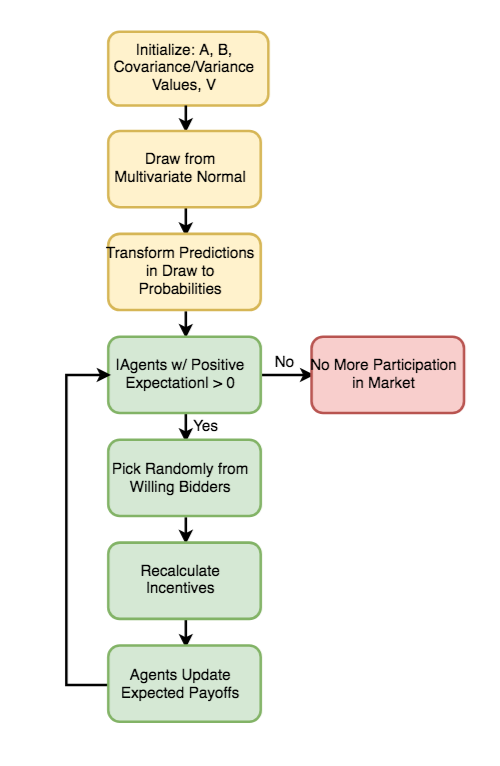
\includegraphics[width=0.4\textwidth]{flow1}
\caption{Simulation Workflow for Strict Incentive Scheme}
\end{figure}

\textit{Market Simulation}\\

Note that from the result by LP in \cite{3}, the expected group prediction error is undefined for a group of size 0 ($M = 0$). Therefore, we cannot apply our additional incentive to the first market participant. We assume arbitrarily to know the type of the first market participant. In reality, this would simply introduce an "off-by-one" error in our estimation of the expected group error.\\

The first participant is selected randomly from the pool of available participants, all of whom have no additional incentive or disincentive to participate. From there, the market organizer calculates the incentives and appropriate $C$ such that the less desirable type for the current state of the market is totally disincentivized from joining per the proposed scheme. Given the newly updated set of incentives, the remaining individuals that have not yet bid recalculate their expected payoffs and choose to remain in the available bidding pool if their payoff is greater than 0. The market simulation terminates when the available pool of willing participants has size 0.\\

The following are a couple assumptions to note about the simulation. First, the choice to choose randomly from the pool enforces arrival to market happens in a random order; there are no high-speed traders in this market. Second, information is integrated into the market immediately and each bidder can update their choice to participate instantaneously.

\subsubsection{Results for Strict Incentive Scheme}

Below in Figure 2, one can see participation proportions and incentives for a single simulation.

\begin{figure}[h]
\centering
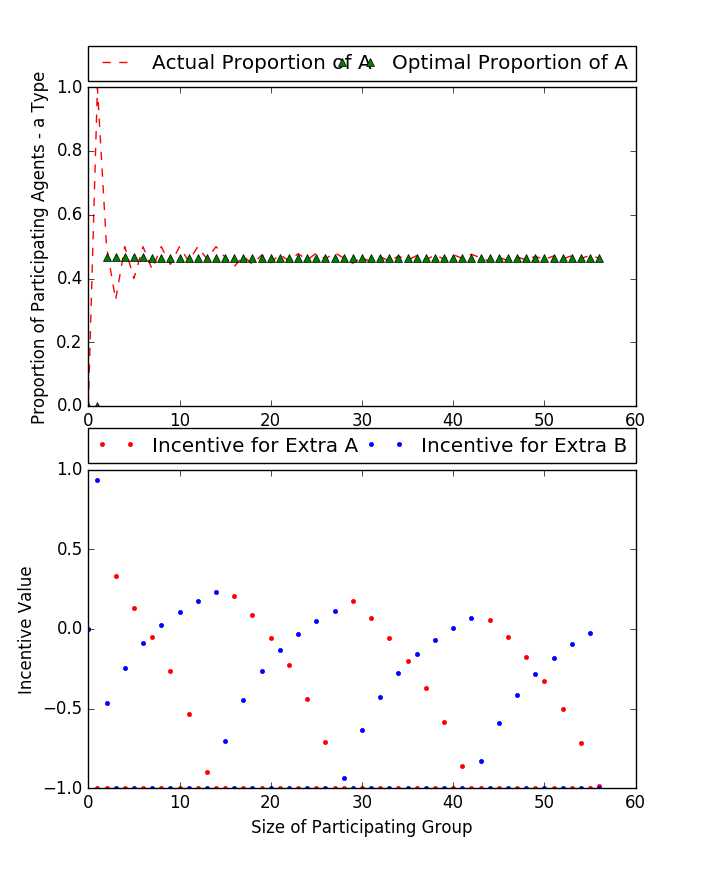
\includegraphics[width=0.45\textwidth]{figure_2.png}
\caption{Market Simulation: A=200, B=100}
\end{figure}

From the simulation, one can see the incentive working in the first subplot. As the crowd gets larger, the actual proportions of the crowd adhere to the optimal proportions related to the covariance and variance statistics of the two types. However, one also notices that the market simulation terminated prior to everyone participating, since the total number of participants does not reach 300. Below, for the same point along the horizontal axis, we see that the incentives for both types for that crowd size in that simulation are both close to -1. Since the actual crowd proportions approach the optimal crowd proportions as the crowd gets larger, a slight deviation in the form of including another individual of either type will leave the crowd in a worse state. However, we know from LP \cite{3} that as the size of the crowd gets larger, expected group error decreases. Here, the market is halting at a local minimum expected error. To prevent this from happening, we will try to relax the incentive scheme to increase market liquidity.

\subsection{Relaxed Incentive Scheme}

The two most salient issues with the strict incentive scheme above is the reliance on severe incentives to exclude a particular type and a lack of liquidity as the size of the participating pool increases. We would like to propose a way to relax these incentives while knowing the types of the individuals that are included in the participating pool. If the incentives for both types are greater than -1, that leaves the possibility that both types could participate. Therefore, the market organizer will need to elicit the types from the agents themselves, and the incentive scheme must guarantee that it is always in the best interests of each agent to report their type truthfully.\\

Previously, the scheme made the payoff for any market participant proportional to the accuracy and sharpness of their prediction as well as their effect on the expected accuracy of the group prediction. Had the individuals been asked to self-report types, there would be no incentive to either lie or tell the truth, since the incentives are not linked to their reported type but to their actual type. To ensure that there is a strict incentive to tell the truth, we propose the following addition to the scheme from earlier.
\newline

\resizebox{0.45 \textwidth}{!}{
$
\pi_i(\vec{p}, \theta) = G(\vec{p}) + C[GE(A,B) - GE(A+1,B)] - \sum_{j>i} e^{-j} \Delta GE_j \ if \ \theta=a
$
}\\

\resizebox{0.45 \textwidth}{!}{
$
\pi_i(\vec{p}, \theta) = G(\vec{p}) + C[GE(A,B) - GE(A,B+1)] -  \sum_{j>i} e^{-j} \Delta GE_j\ if \ \theta=b
$
}\\
\newline

where $j$ indicates an agent that participates after the current agent $i$ participates. Furthermore, $\Delta GE_j$ is short for the change in expected group error following the inclusion of $j$. If $\Delta GE_j > 0$, expected group error increased, hence the subtraction of this term from the expected payoff.\\

This term will reward current participants in the market if future participants bring the expected group error down as well. This term provides agent $i$ with a positive incentive to report their type truthfully. If the agent reports untruthfully, it does not affect that agent in the near term but it will skew the known proportions in the crowd such that future agents cannot make fully-informed decisions as to whether or not they are of the right type for the market at that moment. This could lead to the inclusion of the wrong type at a particular stage in the market after $i$ has participated.







%------------------------------------------------


%------------------------------------------------
\section{Results}



\section{Discussion}

\subsection{Subsection One}

A statement requiring citation \cite{Figueredo:2009dg}.
\blindtext % Dummy text

\subsection{Subsection Two}

\blindtext % Dummy text

\begin{table}
\caption{Example table}
\centering
\begin{tabular}{llr}
\toprule
\multicolumn{2}{c}{Name} \\
\cmidrule(r){1-2}
First name & Last Name & Grade \\
\midrule
John & Doe & $7.5$ \\
Richard & Miles & $2$ \\
\bottomrule
\end{tabular}
\end{table}

%----------------------------------------------------------------------------------------
%	REFERENCE LIST
%----------------------------------------------------------------------------------------

\begin{thebibliography}{99} % Bibliography - this is intentionally simple in this template

\bibitem [1]{1}
J. Wolfers and E. Zitzewitz. Prediction markets. \textit{The Journal of Economic Perspectives},
18(2):107-126, 2004.
\bibitem [2]{2}
 Joyce Berg, Robert Forsythe, Forrest Nelson, and Thomas Rietz. \textit{Results from
a Dozen Years of Election Futures Markets Research}, volume 1 of \textit{Handbook of
Experimental Economics Results}, chapter 80, pages 742-751. Elsevier, 2008.
\bibitem [3]{3}
P. J. Lamberson, Scott E. Page, (2012) \textit{Optimal Forecasting Groups}. \textit{Management Science} 58(4):805-810
\bibitem [4]{4}
Tilmann Gneiting and Adrian E. Raftery. Strictly proper scoring rules, prediction,
and estimation. \textit{Journal of the American Statistical Association}, 102(477):359-378,
March 2007.

 
\end{thebibliography}

%----------------------------------------------------------------------------------------

\end{document}
